% Options for packages loaded elsewhere
% Options for packages loaded elsewhere
\PassOptionsToPackage{unicode}{hyperref}
\PassOptionsToPackage{hyphens}{url}
\PassOptionsToPackage{dvipsnames,svgnames,x11names}{xcolor}
%
\documentclass[
  french,
  11pt,
]{article}
\usepackage{xcolor}
\usepackage{amsmath,amssymb}
\setcounter{secnumdepth}{5}
\usepackage{iftex}
\ifPDFTeX
  \usepackage[T1]{fontenc}
  \usepackage[utf8]{inputenc}
  \usepackage{textcomp} % provide euro and other symbols
\else % if luatex or xetex
  \usepackage{unicode-math} % this also loads fontspec
  \defaultfontfeatures{Scale=MatchLowercase}
  \defaultfontfeatures[\rmfamily]{Ligatures=TeX,Scale=1}
\fi
\usepackage{lmodern}
\ifPDFTeX\else
  % xetex/luatex font selection
  \setmainfont[]{Calibri}
\fi
% Use upquote if available, for straight quotes in verbatim environments
\IfFileExists{upquote.sty}{\usepackage{upquote}}{}
\IfFileExists{microtype.sty}{% use microtype if available
  \usepackage[]{microtype}
  \UseMicrotypeSet[protrusion]{basicmath} % disable protrusion for tt fonts
}{}
\makeatletter
\@ifundefined{KOMAClassName}{% if non-KOMA class
  \IfFileExists{parskip.sty}{%
    \usepackage{parskip}
  }{% else
    \setlength{\parindent}{0pt}
    \setlength{\parskip}{6pt plus 2pt minus 1pt}}
}{% if KOMA class
  \KOMAoptions{parskip=half}}
\makeatother
% Make \paragraph and \subparagraph free-standing
\makeatletter
\ifx\paragraph\undefined\else
  \let\oldparagraph\paragraph
  \renewcommand{\paragraph}{
    \@ifstar
      \xxxParagraphStar
      \xxxParagraphNoStar
  }
  \newcommand{\xxxParagraphStar}[1]{\oldparagraph*{#1}\mbox{}}
  \newcommand{\xxxParagraphNoStar}[1]{\oldparagraph{#1}\mbox{}}
\fi
\ifx\subparagraph\undefined\else
  \let\oldsubparagraph\subparagraph
  \renewcommand{\subparagraph}{
    \@ifstar
      \xxxSubParagraphStar
      \xxxSubParagraphNoStar
  }
  \newcommand{\xxxSubParagraphStar}[1]{\oldsubparagraph*{#1}\mbox{}}
  \newcommand{\xxxSubParagraphNoStar}[1]{\oldsubparagraph{#1}\mbox{}}
\fi
\makeatother


\usepackage{longtable,booktabs,array}
\newcounter{none} % for unnumbered tables
\usepackage{calc} % for calculating minipage widths
% Correct order of tables after \paragraph or \subparagraph
\usepackage{etoolbox}
\makeatletter
\patchcmd\longtable{\par}{\if@noskipsec\mbox{}\fi\par}{}{}
\makeatother
% Allow footnotes in longtable head/foot
\IfFileExists{footnotehyper.sty}{\usepackage{footnotehyper}}{\usepackage{footnote}}
\makesavenoteenv{longtable}
\usepackage{graphicx}
\makeatletter
\newsavebox\pandoc@box
\newcommand*\pandocbounded[1]{% scales image to fit in text height/width
  \sbox\pandoc@box{#1}%
  \Gscale@div\@tempa{\textheight}{\dimexpr\ht\pandoc@box+\dp\pandoc@box\relax}%
  \Gscale@div\@tempb{\linewidth}{\wd\pandoc@box}%
  \ifdim\@tempb\p@<\@tempa\p@\let\@tempa\@tempb\fi% select the smaller of both
  \ifdim\@tempa\p@<\p@\scalebox{\@tempa}{\usebox\pandoc@box}%
  \else\usebox{\pandoc@box}%
  \fi%
}
% Set default figure placement to htbp
\def\fps@figure{htbp}
\makeatother



\ifLuaTeX
\usepackage[bidi=basic,shorthands=off]{babel}
\else
\usepackage[bidi=default,shorthands=off]{babel}
\fi
\ifPDFTeX
\else
\babelfont{rm}[]{Calibri}
\fi
\ifLuaTeX
  \usepackage{selnolig} % disable illegal ligatures
\fi


\setlength{\emergencystretch}{3em} % prevent overfull lines

\providecommand{\tightlist}{%
  \setlength{\itemsep}{0pt}\setlength{\parskip}{0pt}}



 


\usepackage{fontspec}
\usepackage{xcolor}
\usepackage{graphicx}
\usepackage{eso-pic}
\usepackage{changepage}
\usepackage{tikz}
\usepackage{sectsty}
\usepackage{typearea}
\usepackage{pdflscape}
\usepackage{hyperref}
\usepackage{ulem} % Pour le sous-lignage

\usepackage{titlesec}
\definecolor{color_orange}{RGB}{227,108,10} % Définit la couleur orange foncé du chapitre
\definecolor{color_grey}{RGB}{128,128,128} % Définit la couleur grise du titre partie
\definecolor{color_purple}{RGB}{102,0,102} % Définit la couleur mauve pour le titre sous partie.
\definecolor{color_black}{RGB}{0,0,0} % Définit la couleur mauve pour le titre sous partie.

\definecolor{head_color}{RGB}{250,192,144} % Définit la couleur orange clair pour l'en tête.

\usepackage[a4paper, margin=1in]{geometry} % Configure les marges de la page

% modification de l'en-tête
\usepackage[automark]{scrlayer-scrpage}
\clearpairofpagestyles % Efface les configurations d'en-tête et de pied de page par défaut
\ihead{} %titre du document
\addtokomafont{pagehead}{\normalfont\fontsize{8pt}{10pt}\selectfont} %taille de l'en-tête
\addtokomafont{pagehead}{\color{head_color}} % couleur de l'en-tête 

% modification du pied de page

\ifoot{Observatoire de l’environnement en Nouvelle-Calédonie. OEIL \\
12 rue Tourville 98800 Nouméa - Tél. / Fax : 23 69 69 - \href{http://www.oeil.nc}{www.oeil.nc}} % Pied de page à gauche
\addtokomafont{pagefoot}{\normalfont\fontsize{8pt}{10pt}\selectfont} % taille du pied de page
\addtokomafont{pagefoot}{\color{color_grey}} % couleur du pied de page

% modification de la position des numéro de page
\cfoot*{} 
\ofoot*{\pagemark} 
\setkomafont{pagenumber}{\normalfont} % numéro des pages 

\usepackage{float}
\floatplacement{table}{H}  %positionne les tableaux comme défini dans le script

\renewcommand{\thesection}{\Roman{section}}
\renewcommand{\thesubsection}{\thesection.\arabic{subsection}}
\renewcommand{\thesubsubsection}{\thesubsection.\arabic{subsubsection}}
\renewcommand{\theparagraph}{\thesubsubsection.\alph{paragraph}}
\renewcommand{\thesubparagraph}{\roman{subparagraph}.\hspace{1.5em}}

%modification des titres pour appliquer la version OEIL
\titleformat*{\section}{\normalfont\fontsize{14pt}{19pt}\selectfont\color{color_orange}} % chapitre
\titleformat*{\subsection}{\normalfont\fontsize{12pt}{19pt}\selectfont\color{color_grey}} % Titre partie
\titleformat*{\subsubsection}{\normalfont\fontsize{11pt}{19pt}\selectfont\bfseries\itshape\color{color_purple}} %titre sous partie
\titleformat*{\paragraph}{\normalfont\fontsize{11pt}{19pt}\selectfont\bfseries\itshape\color{color_black}} %titre sous partie
\titleformat*{\subparagraph}{\normalfont\fontsize{11pt}{19pt}\selectfont\itshape\color{color_black}} %titre sous partie
\titlespacing*{\subparagraph}{2em}{1.25ex plus 10ex minus .1ex}{\baselineskip}
\usepackage{soul}
\sethlcolor{yellow}
\makeatletter
\@ifpackageloaded{caption}{}{\usepackage{caption}}
\AtBeginDocument{%
\ifdefined\contentsname
  \renewcommand*\contentsname{Table des matières}
\else
  \newcommand\contentsname{Table des matières}
\fi
\ifdefined\listfigurename
  \renewcommand*\listfigurename{Liste des Figures}
\else
  \newcommand\listfigurename{Liste des Figures}
\fi
\ifdefined\listtablename
  \renewcommand*\listtablename{Liste des Tables}
\else
  \newcommand\listtablename{Liste des Tables}
\fi
\ifdefined\figurename
  \renewcommand*\figurename{Figure}
\else
  \newcommand\figurename{Figure}
\fi
\ifdefined\tablename
  \renewcommand*\tablename{Table}
\else
  \newcommand\tablename{Table}
\fi
}
\@ifpackageloaded{float}{}{\usepackage{float}}
\floatstyle{ruled}
\@ifundefined{c@chapter}{\newfloat{codelisting}{h}{lop}}{\newfloat{codelisting}{h}{lop}[chapter]}
\floatname{codelisting}{Listing}
\newcommand*\listoflistings{\listof{codelisting}{Liste des Listings}}
\makeatother
\makeatletter
\makeatother
\makeatletter
\@ifpackageloaded{caption}{}{\usepackage{caption}}
\@ifpackageloaded{subcaption}{}{\usepackage{subcaption}}
\makeatother
\usepackage{bookmark}
\IfFileExists{xurl.sty}{\usepackage{xurl}}{} % add URL line breaks if available
\urlstyle{same}
\hypersetup{
  pdfauthor={Hugo Roussaffa},
  pdflang={fr},
  colorlinks=true,
  linkcolor={blue},
  filecolor={Maroon},
  citecolor={Blue},
  urlcolor={Blue},
  pdfcreator={LaTeX via pandoc}}


\author{Hugo Roussaffa}
\date{24 juillet 2026}
\begin{document}
% Script LaTex pour la mise en forme de la page de garde

\definecolor{titreColor}{RGB}{227, 108, 10} %orange titre
\definecolor{grey_color}{RGB}{128, 128, 128} %gris pour auteur et editeur
\definecolor{date_color}{RGB}{227, 150, 70} % orange clair pour la date
\definecolor{version_color}{RGB}{102, 0, 102} %mauve pour le versionning du rapport

\noindent

%ajout de l'image de fond 
\begin{titlepage}
    \vspace*{-18.18cm}
    \hspace*{-5.7cm}
    \begin{tikzpicture}
        \clip [rounded corners=60pt] (0,2cm) rectangle (23.5cm,26cm); %arrondissement des bords d'image
        \node[inner sep=0pt, anchor=south west] at (0,0) {
            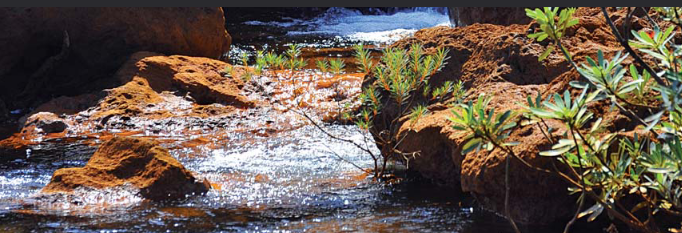
\includegraphics[width=27cm,height=16cm]{../ressources/MJunckerOEIL.jpg}
        };
    \end{tikzpicture}

    %ajout de l'image supérieur
    \begin{tikzpicture}[remember picture, overlay]
        \clip [rounded corners=30pt] (-0.5cm,-2.5cm) rectangle ++(9cm,5.5cm);
        \node[inner sep=0pt, anchor=south west] at (-0.5cm,-2.5cm) { 
            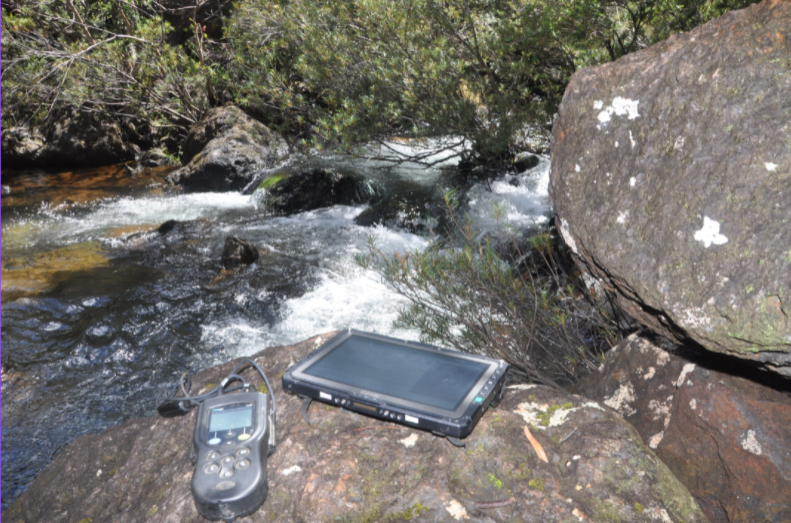
\includegraphics[width=10.5cm,height=6.5cm]{../ressources/eau-monitoring.png}
        };
        \draw [white, line width=3pt, rounded corners=30pt] (-0.5cm,-2.5cm) rectangle ++(9cm,5.5cm); %trait blanc autour de l'image
    \end{tikzpicture}

    %ajout du versionning du rapport
    \begin{minipage}[2cm]{16cm}
        \begin{adjustwidth}{12cm}{1cm} 
            \vspace{0.5cm}
            {\fontsize{10}{12}\selectfont
            \color{version_color}
            
            }
        \end{adjustwidth}
    \end{minipage}

% intégration des titre, sous-titre, auteurs et date
    \begin{minipage}[2cm]{16cm}
        \begin{adjustwidth}{0.5cm}{1cm} 
            \vspace{2.2cm}
            {\fontsize{16}{20}\selectfont
            \color{titreColor}
            \\
            }
            {\fontsize{10}{20}\selectfont
            \color{titreColor}
            \\
            }

            {\fontsize{12}{14}\selectfont
            \color{grey_color}
            Hugo Roussaffa\\
            \\
            }
    
            {\fontsize{12}{8}\selectfont
            \color{date_color}
            24 juillet 2026\\
            }

        \end{adjustwidth}
    \end{minipage}

    %ajout du logo OEIL
    \begin{tikzpicture}[remember picture,overlay]
        \node [inner sep=0pt] at (12.5cm,-4.8cm) {\includegraphics[width=4.5cm,height=5.5cm]{../ressources/OEIL\_logo.png} 
        };
    \end{tikzpicture}

    %ajout d'element supplémentaire ou logo partenaire
    \begin{minipage}[1cm]{16cm}
        \begin{adjustwidth}{-0.4cm}{1cm} 
            \vspace{3.4cm}
            \begin{tikzpicture}[remember picture,overlay]
                \node [inner sep=0pt] at (12.5cm,-5cm) {\includegraphics[width=7cm,height=1.5cm]{../ressources/logo\_yapuka.png} 
            };
            \end{tikzpicture}
            {\fontsize{11}{13}\selectfont
            \color{version_color}
            \\  \\ Nouvelle-Calédonie\\  % ou Logo partenaire/prestataire H, 5.5cm
            }
        \end{adjustwidth}
    \end{minipage}

\end{titlepage}

\renewcommand*\contentsname{Table des matières}
{
\setcounter{tocdepth}{3}
\tableofcontents
}

\section{Définition du cadre opérationnel du
projet}\label{duxe9finition-du-cadre-opuxe9rationnel-du-projet}

\subsection{Périmètre du projet}\label{puxe9rimuxe8tre-du-projet}

Le projet s'articule autour de quatre domaines :

\begin{itemize}
\tightlist
\item
  Connaissance et caractérisation du territoire;
\item
  Diagnostic et analyse multicritère;
\item
  Veille et détection automatique des changements;
\item
  Partage et diffusion des diagnostics;
\end{itemize}

\subsubsection{Logique de délimitation du périmètre vis à vis des
besoins
remontés}\label{logique-de-duxe9limitation-du-puxe9rimuxe8tre-vis-uxe0-vis-des-besoins-remontuxe9s}

Pour apporter de la transparence aux processus de vérification et
d'intégration des fonctionnalités dans le périmètre d'Hydroscope, nous
définissons 3 critères. Par exemple, une fonctionnalité ou une donnée
est incluse si elle répond à toutes les conditions suivantes :

\begin{itemize}
\tightlist
\item
  \textbf{Elle produit une information utile à la décision sur la
  ressource en eau potable} :
\end{itemize}

L'outil n'a pas vocation à centraliser toute l'information disponible
sur le territoire --- uniquement celle qui permet de caractériser une
pression, d'évaluer une vulnérabilité ou d'orienter une action de
protection sur la ressource en eau potable.

\begin{itemize}
\tightlist
\item
  \textbf{Elle est techniquement soutenable dans le temps}:
\end{itemize}

Les données intégrées doivent pouvoir être actualisées de manière
récurrente et maîtrisée. Une donnée pertinente mais trop instable, trop
dépendante d'un tiers ou trop coûteuse à maintenir est exclue pour ne
pas fragiliser la fiabilité de l'ensemble du système.

\begin{itemize}
\tightlist
\item
  \textbf{Elle relève du périmètre de responsabilité de l'OEIL}:
\end{itemize}

Hydroscope ne se substitue pas aux systèmes existants gérés par d'autres
acteurs. Lorsqu'une information est déjà produite et gérée par un
partenaire dans un système dédié, l'outil peut s'y connecter ou en
restituer une synthèse --- mais il ne reprend pas la responsabilité de
sa production ni de sa mise à jour.

\subsubsection{Ce qui est exclu du périmètre --- cadre et
justifications}\label{ce-qui-est-exclu-du-puxe9rimuxe8tre-cadre-et-justifications}

Afin d'évaluer des cas plus précisément, les critères exclusifs suivant
seront aussi évalués.

\begin{itemize}
\tightlist
\item
  \textbf{Les données internes propres à chaque partenaire}:
\end{itemize}

Hydroscope est un outil de diagnostic territorial partagé, construit sur
des référentiels communs et validés collectivement. Il n'a pas vocation
à intégrer des bases de données locales, des tableurs ou des systèmes
internes propres à chaque structure. Une telle intégration créerait une
dépendance à des sources non maîtrisées, non standardisées et non
pérennes, compromettant la fiabilité de l'ensemble du système. Si une
donnée produite par un partenaire présente une valeur territoriale
réelle, la voie appropriée est sa formalisation en référentiel partagé
--- ce qui relève d'un processus distinct, piloté par les acteurs
concernés.

\begin{itemize}
\tightlist
\item
  \textbf{Les fonctionnalités de gestion et de saisie}:
\end{itemize}

Hydroscope est un outil de lecture et d'analyse statistique --- pas un
système de gestion documentaire, de suivi de dossiers ou de workflow
administratif. Intégrer des fonctionnalités de saisie, de validation ou
de suivi de procédures dépasserait le périmètre fonctionnel du projet et
alourdirait considérablement la complexité technique et les coûts de
maintenance. Ces besoins, légitimes en eux-mêmes, relèvent d'autres
outils métiers existants ou à développer séparément.

\begin{itemize}
\tightlist
\item
  \textbf{Les données sensibles et confidentielles}:
\end{itemize}

L'accès aux données brutes physico-chimiques, de météorologie ou de
recencement, aux valeurs précises de mesures ou à toute information
soumise à des restrictions de confidentialité est exclu du périmètre.
Cet arbitrage protège à la fois les partenaires producteurs de ces
données et l'OEIL, en maintenant des périmètres de responsabilité
clairs. Hydroscope restitue des indicateurs agrégés et des informations
de présence --- jamais les données sources sensibles elles-mêmes.

\begin{itemize}
\tightlist
\item
  \textbf{La vulgarisation pédagogique et la communication grand public
  approfondie}:
\end{itemize}

La sensibilisation citoyenne, la narration pédagogique et la
communication narrative sont prises en charge par le projet partenaire
SOURCE, avec lequel Hydroscope est coordonné. Développer ces
fonctionnalités dans Hydroscope créerait une redondance coûteuse et un
risque d'incohérence dans les messages diffusés. L'interface Grand
Public d'Hydroscope fournit une information accessible et cartographiée
--- elle ne se substitue pas à une démarche de communication structurée.

\begin{itemize}
\tightlist
\item
  \textbf{Fonctionnalités à fort impact budgétaire ou de maintenance}:
\end{itemize}

Au-delà des exclusions thématiques, certaines demandes peuvent sembler
compatibles avec les objectifs du projet mais engendrer des coûts de
développement ou de maintenance disproportionnés par rapport à la valeur
produite. Ces demandes sont également écartées du périmètre,
indépendamment de leur pertinence fonctionnelle.

Trois situations typiques sont identifiées :

\begin{itemize}
\tightlist
\item
  \textbf{Le développement sur-mesure pour un usage isolé}:
\end{itemize}

Une fonctionnalité utile à un seul partenaire, dans un contexte
spécifique, ne justifie pas un développement dédié. Le coût de
conception, de test et de maintenance d'une fonctionnalité marginale est
sans commune mesure avec sa valeur pour l'ensemble du système.
Hydroscope est conçu pour répondre à des besoins partagés --- pas pour
agréger des cas particuliers.

\begin{itemize}
\tightlist
\item
  \textbf{Les connecteurs et intégrations techniques non standardisés}:
\end{itemize}

Connecter Hydroscope à un système tiers mal documenté, propriétaire ou
instable crée une dette technique immédiate. Chaque mise à jour du
système tiers peut casser l'intégration et mobiliser des ressources de
maintenance non provisionnées. Seules les intégrations reposant sur des
protocoles ouverts et stables sont envisageables.

\begin{itemize}
\tightlist
\item
  \textbf{Les fonctionnalités temps réel ou à haute fréquence de mise à
  jour}:
\end{itemize}

L'automatisation des flux de données est prévue dans le projet, mais
elle est calibrée sur des cycles cohérents avec la nature des pressions
suivies --- hebdomadaires ou mensuels selon les cas. Des demandes de
mise à jour en temps réel ou quasi temps réel impliquent une
infrastructure et des coûts d'exploitation sans rapport avec les besoins
opérationnels identifiés dans le projet.

\subsubsection{Ce que ce cadre implique pour les demandes
d'évolution}\label{ce-que-ce-cadre-implique-pour-les-demandes-duxe9volution}

Toute demande d'intégration d'une nouvelle fonctionnalité ou donnée sera
évaluée selon ces critères, de son impact budgétaire et de maintenance.
Une demande qui n'y répond pas n'est pas rejetée définitivement --- elle
est documentée et pourra être réexaminée si les conditions changent. Les
arbitrages finaux relèvent de l'OEIL.

\subsection{Hypothèses et
contraintes}\label{hypothuxe8ses-et-contraintes}

\subsubsection{Disponibilité et la fiabilité des
données}\label{disponibilituxe9-et-la-fiabilituxe9-des-donnuxe9es}

La réussite du projet repose en grande partie sur l'accès aux données
fournies par les partenaires institutionnels et privés (Gouvernement,
Provinces, Communes, DASS, ISEE, CDE).

Le projet doit s'assurer de l'interopérabilité entre les référentiels
des partenaires, la DAVAR, de la DITTT (BD-Hydrographie, BDTOPO), de
l'ISEE (statistiques de population), des réseaux de distribution d'eau
potable (SERAIL, communes, CDE) etc. L'interopérabilité ne dépend pas
seulement de la technique d'Hydroscope, mais aussi de la coopération des
partenaires (DAVAR, DITTT, ISEE, CDE) et de la conformité de leurs
propres référentiels. L'équipe projet va vérifier et garantir que les
conditions sont réunies pour que les systèmes puissent se connecter en
sécurisant les liens avec les partenaires.

Voici une liste des référentiels hydrologiques produits par des acteurs
en Nouvelle-Calédonie :

\begin{itemize}
\tightlist
\item
  BD-Hydrographie (DITTT);
\item
  Cartographie des Bassins Versants d'Approvisionnement en Eau Potable
  (BVAEP) de la DAVAR;
\item
  Cartographie des Périmètres de Protection des Eaux de la DAVAR;
\item
  Positionnement des captages destinés à l'Alimentation en Eau Potable
  de la DAVAR;
\item
  Cartographie des Hydro-Eco Régions;
\end{itemize}

Des référentiels non hydrologiques produits en Nouvelle-Calédonie
pourront être exploités :

\begin{itemize}
\tightlist
\item
  Pluviométrie (Météo France NC);
\item
  Statistiques de population (ISEE);
\item
  Incendies (OEIL);
\item
  Plans Locaux d'Urbanisme (Provinces);
\item
  Base de données des ICPE (DIMENC, Provinces);
\item
  Réseau de distribution d'eau potable (SERAIL, communes, CDE); ainsi
  que des fonds de plans cartographique et d'imagerie de la DTSI;
\end{itemize}

D'autres référentiels hydrologiques et non hydrologiques produit en
dehors de la Nouvelle-Calédonie pourront être exploités :

\begin{itemize}
\tightlist
\item
  Dynamic world : artificialisation des sols ;
\item
  TMF: évolution du couvert forestier;
\end{itemize}

La liste des ressources utiles au projet est à compléter et à valider
lors des ateliers de cadrage fonctionnel. Les partenaires et acteurs
institutionnels doivent s'engager activement dans la validation des
indicateurs et la définition des seuils de vigilance, garantissant ainsi
l'appropriation du diagnostic territorial partagé.

\subsubsection{Ressources humaines}\label{ressources-humaines}

Les ressources internes de l'OEIL, que ce soit au pôle Environnement
qu'au pôle Système d'Information peuvent assurer la production du
projet. Cependant, il sera nécessaire de prévoir des ressources externes
pour la réalisation technique (Phase B) et probablement pour la
maintenance post-livraison, notamment pour l'hébergement cloud ainsi que
l'automatisation des traitements.

\begin{center}\rule{0.5\linewidth}{0.5pt}\end{center}

\newpage{}

\section{Les ateliers de collecte des besoins}\label{sec-ateliers}

Les ateliers métiers du projet Hydroscope, prévus durant la Phase A
(mi-avril à mi-mai 2026), constituent une étape pivot pour passer de la
vision stratégique aux spécifications techniques. Ils visent à
recueillir les besoins des partenaires tout en garantissant que l'outil
reste aligné sur les objectifs du projet porté par l'OEIL.

\subsection{Objectifs des ateliers}\label{objectifs-des-ateliers}

Le premier objectif est de \textbf{recueillir et centraliser les besoins
fonctionnels} d'une majorité d'acteurs sur le territoire pour construire
une vision partagée de la ressource.

Les ateliers permettront de définir :

\begin{itemize}
\tightlist
\item
  Les indicateurs prioritaires et leur valeur métier;
\item
  Les profils utilisateurs et leurs besoins spécifiques (gestionnaires,
  partenaires, grand public);
\item
  Les fonctionnalités attendues pour chaque profil (navigation,
  visualisation cartographique, tableaux de bord, filtres, exports,
  ergonomie, niveau de complexité attendu);
\item
  Les contraintes opérationnelles et réglementaires;
\item
  Les seuils de vigilance et d'alerte des indicateurs;
\item
  Les besoins de partage et de collaboration entre acteurs;
\item
  les modalités d'accès aux données (API, exports, interfaces);
\item
  les contraintes d'usage (fréquence de mise à jour, fréquence
  d'utilisation de l'outil, performance, besoin d'autonomie ou
  d'accompagnement, accessibilité).
\end{itemize}

\textbf{Animation et synthèse :}

Les ateliers sont animés par l'assistance à maîtrise d'ouvrage (AMOA),
qui est chargée de la rédaction des comptes rendus. Ces derniers sont
ensuite \textbf{validés par l'OEIL} pour assurer la cohérence avec les
objectifs globaux.

\textbf{Arbitrage final :}

L'équipe projet synthétise ensuite l'ensemble des besoins recueillis
pour préparer les arbitrages finaux du \textbf{COPIL}, garantissant que
les choix retenus respectent le périmètre du projet.

Pour légitimer ces sollicitations, l'OEIL pourrait demander une
\textbf{lettre de mission officielle} auprès du Gouvernement, facilitant
ainsi la mobilisation des services techniques partenaires.




\end{document}
